% !TEX root = diss.tex

 \chapter{Introduction}

Radicals are chemical species which tend to be highly reactive due to the presence of one or more unpaired electrons. Living systems depend on radical processes as part of normal metabolism but biomaterials such as proteins, are susceptible to radical induced damage. Radical induced oxidation of biomaterials has been implicated in a number of degenerative disease states, including cancer, Alzheimer's Disease, Parkinson's Disease, and multiple sclerosis.\cite{Barnham2004,Halliwell2007,Valko2007,Hwang2013,Halliwell2015}

In biological systems, radicals are derived from both endogenous sources, such as transition metal-ion redox processes involved in respiration and other \emph{in vivo} processes, as well as exogenous sources, for instance, solar radiation and air pollutants. A significant portion of ROSs originate from reactions of \ch{O2} with the redox-active metals copper and iron,\cite{Halliwell2015} such as those reactions involved in Fenton chemistry.\cite{Stohs1995} Oxygen-centred radicals, known as reactive oxygen species (ROSs) in biology, are particularly important due to the nature of the aerobic respiration. The radicals of primary concern are the highly reactive hydroxyl radical (\ch{HO^.}), alkoxyl radicals (\ch{RO^.}), superoxide (\ch{HOO^.}/\ch{O2^{.-}}), and peroxyl radicals (\ch{ROO^.}).\cite{Halliwell2015} Damage occurs when an ROS initiates a radical chain reaction through hydrogen atom transfer (HAT), electron transfer, or addition reactions, leading to rapid propagation. HAT is the most relevant reaction and is the focus of my work.

This work is primarily concerned with models for proteins. The oxidation of protein by ROSs occurs through a radical chain mechanism which has been studied in detail.\cite{Berlett1997,Davies2016} As there are 20 common amino acid side chains, as well as a common peptide backbone in proteins, there are a large number of possible reactions. Proteins are the most abundant biomaterial in most biological systems,\cite{Davies2005} thus understanding their degradation is essential to understaning degenerative disease. Some of the reactions involved in protein oxidation are shown in~\ref{fig:proteinoxidation}.

\begin{scheme}[H]
  \centering
  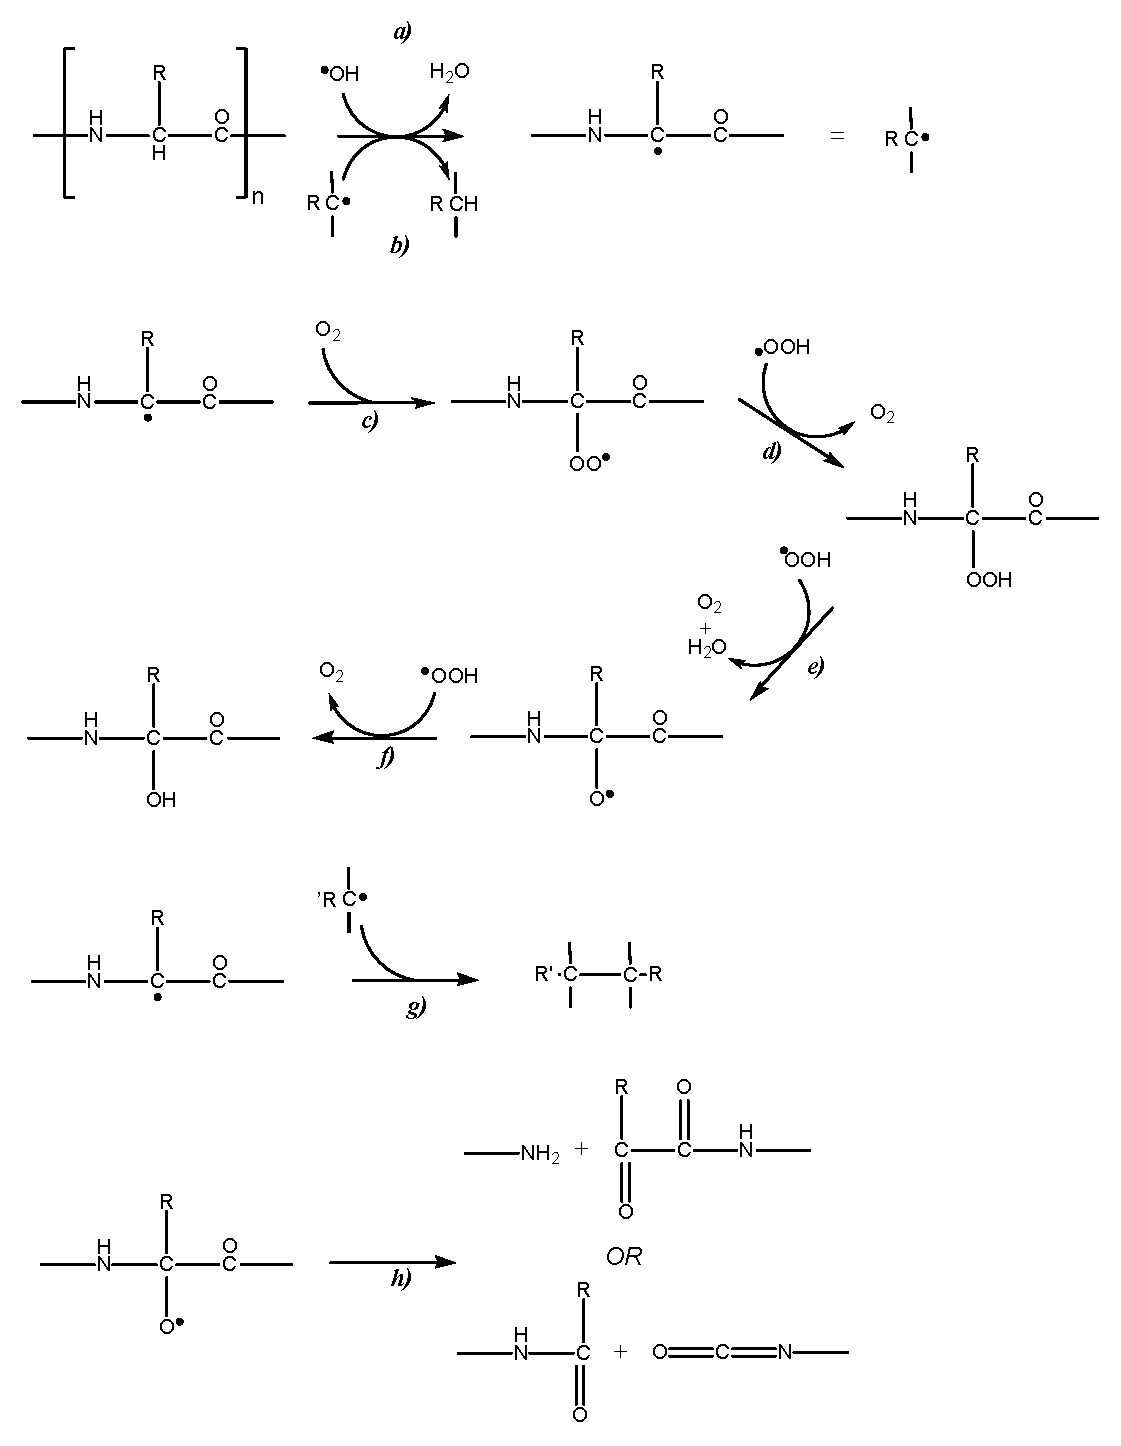
\includegraphics[height=12cm]{figures/proteinoxidation-1.eps}
  \caption[Common reactions involved in the radical-mediated oxidation of proteins]{Common reaction involved in the radical-meditated oxidation of proteins. The reactions are as follows: initiation of radical chain through abstraction by \textbf{a)} the hydroxyl radical \textbf{b)} $\alpha$-carbon radical, \textbf{c)} radical addition of molecular oxygen, \textbf{d)} HAT with an incoming peroxyl radical, \textbf{e)} additional reaction with an incoming peroxyl radical producing water and oxygen, \textbf{f)} formation of hydroxyl-amide by HAT with an incoming peroxyl radical, \textbf{g)} possible cross-linking mechanism of two carbon-centred radicals, \textbf{h)} possible fragmentation pathways of an oxygen-centred radical intermediate. Figure adapted from Reference \protect\citenum{Berlett1997}.}
\label{fig:proteinoxidation}
\end{scheme}

Initial abstraction (Reaction \textbf{a}) often occurs at the $\alpha$-carbon position (\ch{R2CH}), forming a carbon-centred radical (\ch{R2C^.}) which is partially delocalised in the $\pi$-system of the amide group. Many studies have indicated that the stability of \ch{R2C^.} is determined by stereo-electronic considerations related to the planarity of the amide group. For example, steric bulk of the side chains, as well as local protein structure (helix, sheet, etc.) can constrain radical geometries. Therefore, the most captodatively stable $\alpha$-carbon radical occurs at glycine residues in antiparallel $\beta$-sheets.\cite{Rauk2000} The side-chains are also susceptible to oxidation. Those side-chains containing sulphur,\cite{Stadtman2004} as well as tyrosine (which has a fairly weak phenolic O-H bond of about 89 \kcalmol),\cite{Mulder2005} are particularly susceptible to oxidation.

Propagation occurs through various processes, including the abstraction of another H atom by the newly formed \ch{R2C^.} (Reaction \textbf{b}), or radical-mediated oxidation,\cite{Stadtman2003} leading to the formation of an oxidised carbon centre (\ch{R2COH}). The course of propagation through radical-mediated protein oxidation is determined by the availability of either singlet oxygen (\ch{^1O2}), or superoxide (\ch{O2^{.-}}) (or the protonated form, peroxyl radical (\ch{^.OOH})). Those reactions which occur in the presence of \ch{O2} and \ch{^.OOH} are shown in Reactions \textbf{c-f}. The radical chain reaction can be terminated through several mechanisms, including protein-protein cross-linking (Reaction \textbf{g}), protein fragmentation (Reaction \textbf{h}), or through reactions with antioxidants. The sum total of all these processes leads to the accumulation of oxidised proteins which is associated with many degenerative diseases.\cite{Halliwell2006}

\section{Studying HAT reactions}

Formal HAT reactions are a fundamental radical chemical transformation which has been studied for over a century.\cite{Kochi1973,Parsons2000} At the macroscopic level, HAT reactions which involve oxygen-centred radicals and non-radical organic substrates are reasonably well characterised: the effects of bulk solvent are well understood.\cite{Litwinienko2007} However, the roles of substrate-radical and substrate-radical-medium interactions at the microscopic (molecular) level continue to be relatively poorly understood. In my work, I shall make use of quantum chemistry in order to study formal HAT at the molecular level. In doing so, I hope to contribute to a better understanding of the fundamental properties which govern these reactions, and thus develop insights into the many important processes in which HAT takes place.

The potential energy surface (PES) for any chemical reaction is a complex hypersurface that depends on many variables. Typically this problem can be simplified by examining only the relevant geometry changes. Often the two most important coordinates can be isolated, giving a 3-dimensional potential energy surface. Furthermore, in chemistry we simplify this problem to 2-dimensions, such that the so-called intrinsic reaction coordinate, or the lowest energy cross section of a higher dimension PES.\@ This yields a reaction coordinate diagram, as is illustrated below in~\ref{fig:pes}.

\begin{figure}[htb]
  \centering
  \includegraphics[width=0.9\textwidth]{figures/pes-1}
  \caption[Three-dimensional potential energy surface and corresponding reaction coordinate diagram.]{Three-dimensional potential energy surface and corresponding reaction coordinate diagram. Stationary states A, B, and C, correspond to the pre-reaction, transition state, and post-reaction complexes, respectively.}
\label{fig:pes}
\end{figure}

\noindent In a typical reaction coordinate diagram, the reactants begin to interact and form a pre-reaction complex (A). Given sufficient energy, the reaction will proceed over the top of the energy barrier through a transition state (TS) complex (B). After the chemical transformation is completed, a post-reaction complex (C) is formed until the products are able to separate.

In quantum chemistry, we are generally concerned with the thermodynamic and kinetic properties of a reaction. This is achieved through the investigation of stationary states (reactants, pre-reaction complex, TS complex, post-reaction complex, and products) along the reaction coordinate. Thermodynamic analysis of a reaction requires the understanding of the stability of the products relative to the reactants, measured by change in Gibbs free energy $\Delta G$, while kinetic analysis requires the understanding of the stability of the TS complex relative to the reactants measured by the Gibbs free energy barrier $\Delta G^{\ddagger}$.

To fully understand HAT reactions, one must analyse the factors which influence the thermodynamics and kinetics of these reactions. Thermodynamically this is relatively simple; relative bond strengths generally dictate the stability of products relative to reactants for HAT reactions. Typically, a reaction will be exergonic if the bond being formed is stronger than the bond being broken. Entropic changes ($\Delta S$) in HAT reactions are in all but the most unusual cases, negligible ($\Delta S \approx 0$).\cite{Mader2007} Kinetic analysis can be considerably more complicated, as there are numerous factors which can stabilise or destabilise the reactants or TS complex. I have investigated several fundamental concepts associated with HAT reactions.

Recent work from our group, in collaboration with colleagues at University of Rome Tor Vergata, has focused on the importance of substrate-radical interactions. Specifically, it has been shown that the three-dimensional structures of oxygen-centred radicals, as well as the organic substrates, impacts the nature of the interactions involved in HAT reaction pathways.\cite{Salamone2015Rev} In our work, we utilise primarily the \bno and \cumo radicals, which serve as a convenient proxy to biological oxygen-centred radicals. Reaction involving \bno and \cumo can be easily monitored using highly resolved laser flash photolysis (LFP) techniques. A combination of theoretical and experimental techniques have been used to examine reactions involving \bno and \cumo with a variety of organic substrates. A detailed discussion of these results shall be reserved for following chapters, however, a great deal of insight has been gained into the role of structure in both the radicals and substrates, and resulting intermolecular interactions.

Non-covalent interactions (NCIs; eg.\ van der Waals interactions, hydrogen bonding, etc.)  play a central role in all chemistry. Oxygen-centred radicals can hydrogen bond with substrates as both acceptors and donors.\cite{Johnson2009a} These hydrogen bonding interactions, in addition to the other non-covalent interactions between the radical and substrate lead to the formation of a pre-reaction complex. NCIs are also known to be important in the stabilisation of TS complexes in HAT reactions.\cite{DiLabio2005,DiLabio2007} Although the effects of NCI stabilisation are difficult to quantify, the concept of TS complex stabilisation is being recognised in applications such as enzymatic\cite{Uyeda2011} and synthetic catalysis.\cite{Bakr2016}

In Chapter~\ref{ch:arrhenius}, I shall consider non-covalent binding in the pre-reaction complex with respect to the well known, but phenomenological Arrhenius equation. Arrhenius parameters for the systems of interest in this work were previously tabulated,\cite{DiLabio2005} and consist of thermoneutral or nearly thermoneutral reactions involving the creation and destruction of oxygen-centred radicals. These reactions are related to the phenol-phenoxyl self-exchange reaction in that a relatively strong pre-reaction complex is expected. As of yet, there is no framework which relates the non-covalently bound pre-reaction complex to kinetic results. We ask the simple question: does there exists a direct correlation between the Arrhenius pre-factor and the non-covalent binding energy?

Bond strengths are measured by bond dissociation enthalpies (BDEs), and are central to the understanding of reactivity with respect to thermodynamics. In addition to this, there exists a tremendous amount of literature in which BDEs are linked to chemical reactivity, especially for HAT reactions.\cite{Kochi1973,Tedder1982,Wijtmans2003,Pratt2004,Mayer2004} There exists a linear free energy relationship (LFER), the Bell-Evans-Polanyi (BEP) Principle,\cite{Bell1936,Evans1938} which states that the difference in activation energy ($E_a$) for two related reactions, is proportional to the differences in reaction enthalpy ($\Delta H$):

\begin{equation}
  E_a = E_0 + \alpha \Delta H
  \label{eq:bep}
\end{equation}

\noindent where $E_0$ is the activation energy of a reference reaction, and $\alpha$, a constant which characterises the position of the TS along the reaction coordinate. This relationship can be more generally used to compare larger families of reactions, although the applicability of this relationship is not well described.

In Chapter~\ref{ch:bde} I probe the applicability of the BEP principle, with the aim to determine how generally the BEP principle can be applied. This is achieved by relating highly-accurate, theoretically determined C-H bond strengths of species which undergo abstraction at these positions to the experimentally determined HAT rate constants. HAT reaction rate constants depend on many factors, however, by using measured rate constants from specific conditions (LFP with \cumo at 298K), the difference in reactivity depend mainly on the differences in chemical properties of the systems of interest. Therefore, we hypothesise that there should exist two BEP relationships for abstraction of C-H bonds: one in which the incipient radical is delocalised into a $\pi$-system (benzylic/allylic) and the remaining alkyl radicals which are largely localised.

Finally, recent experimental results show that non-redox active metal cations, which are found ubiquitously in biological systems, have an inhibitory effect on HAT reactions involving oxygen-centred radicals and substrates which undergo abstraction from sites adjacent to heteroatoms (e.g.\ amines, amides, and ethers). Under various stoichiometric ratios, these metal cations have effects ranging from full inhibition to partial deactivation of HAT reactivity.\cite{Salamone2013,Salamone2015metals,Salamone2016} This effect has been attributed partially to the effects of hyperconjugative overlap. Take for example tetrahydrofuran (THF), shown in~\ref{fig:THF}. Normally, there exists C-H bond weakening hyperconjugative overlap of electron density from one of the oxygen lone-pairs and the adjacent C-H $\sigma^*$ anti-bonding orbitals. The interaction of a metal cation with the oxygen lone-pairs removes electron density from this interaction, thus increasing the C-H bond strength. As a results, the reactivity of this bond is decreased, as observed from the experimentally measured 3.2-fold decrease in the rate constant for HAT with \cumo~in acetonitrile from 6.65 \E{7} \Ms to 7.0 \E{7} \Ms in the presence of 1.0 M \ch{Mg(ClO4)2}.\cite{Salamone2013}

\begin{scheme}[htb]
  \centering
  \includegraphics[width=0.65\textwidth]{figures/THF}
  \caption[Hyperconjugative overlap in tetrahydrofuran and the effect of non-redox active metal cations.]
  {Hyperconjugative overlap in tetrahydrofuran and the effect of non-redox active metal cations. The metal cation accepts electron density from the heteroatom lone pair, reducing overlap with the C-H $\sigma^*$ anti-bonding orbital and increasing the C-H bond strength.}
\label{fig:THF}
\end{scheme}

The nature of the interactions between non-redox active metal cations and organic substrates is poorly understood. The primary goal of this thesis is to understand the fundamental physico-chemical properties which lead to the experimentally observed trends in reactivity. This problem is explored in Chapter~\ref{ch:hat}. The experimentally observed effects have led us to hypothesise that the presence of non-redox active metal cations has a chemoprotective effect against the radical induced oxidation of biomaterials such as proteins.

\section{Mechanistic details of hydrogen transfer reactions}

For a simple HAT reaction, there exists several possible mechanisms by which this transformation can occur. The two most common concerted mechanisms are direct HAT\footnotemark~and proton-coupled electron transfer (PCET). At the basic level, direct HAT involves the transfer of an electron and proton through the same set of acceptor/donor orbitals, while PCET involves the transfer of an electron and proton through different sets of orbitals. In practise, this distinction is poorly described and this topic is still in active discussion in the literature.\cite{Cukier1998, Mayer2002, Stubbe2003, Mayer2004, DiLabio2007, Huynh2007, HammesSchiffer2008, Mayer2010, Weinberg2012, HammesSchiffer2015, MunozRugeles2017} Primarily, the distinction between the two processes is unclear because the two processes cannot be entirely separated physically.\cite{DiLabio2007}

\footnotetext{Not to be confused with the net reaction of formal hydrogen atom transfer. The abbreviation HAT will be used interchangeably, although the distinction should be clear from context.}

The quintessential example when comparing direct HAT to PCET is the self-exchange reactions of benzyl/toluene and phenoxyl/phenol shown in~\ref{fig:self1}, as described by \citet{Mayer2002}

\begin{scheme}[htb]
  \textbf{A. }\\
    \includegraphics[width=0.75\textwidth]{figures/PhCH3-PhCH2.eps}\\
 \textbf{B. }\\
    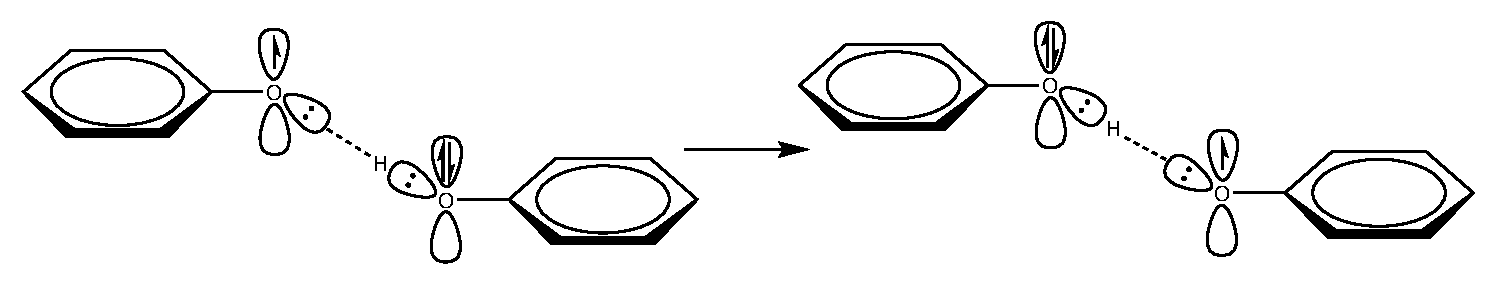
\includegraphics[width=0.95\textwidth]{figures/PhOH-PhO.eps}\\
    \caption{Self-exchange reactions of the \textbf{A.} benzyl/toluene couple
      through direct HAT \textbf{B.} phenoxyl/phenol couple through PCET.}
\label{fig:self1}
\end{scheme}

In this work, the transition state structures, obtained through theoretical studies, were reported. The proposed structures have $C_{2h}$ and $C_2$ symmetry for~\ref{fig:self1} A and B, respectively, oriented so that the aromatic rings are trans relative to one another. In this geometry, the benzyl/toluene pair undergoes direct HAT, with the $2p-\pi$ orbital of the benzylic carbon radical oriented at the benzylic hydrogen on toluene and little delocalisation of the radical into the $\pi$-system. Additionally, the singly occupied molecular orbital (SOMO) is of $\sigma$-symmetry. The calculated enthalpic barrier ($\Delta H^{\ddagger}$) is 17.7 \kcalmol. For the phenoxyl/phenol pair, a fairly strongly hydrogen bonded pre-reaction complex is first formed (-8.1 \kcalmol, relative to reactants).
The TS structure is such that the phenoxyl radical occupies a $2p$ orbital, and is allowed to overlap with the $2p$ lone pair of the phenol moiety and the aromatic $\pi$ systems. This demonstrates that the SOMO is of $\pi$-symmetry and highly delocalised, and that HAT occurs through a PCET mechanism. The reaction has a barrier height $\Delta H^{\ddagger}$ = 5.0 \kcalmol relative to the hydrogen bonded complex, so that the barrier is 3.1 \kcalmol below the separated reactants.

The work by \citet{Mayer2002} suggests that hydrogen bonding is a necessary, but not sufficient condition for PCET to occur. This then implies that PCET is not possible between molecules which do not possess hydrogen bonding moieties, such as carbon atoms. Work by other authors has shown this to be untrue.\cite{Hatcher2007, DiLabio2007} In particular, \citet{DiLabio2007} demonstrated that this neglected the important contributions of $\pi-\pi$ interactions and lone pair-$\pi$ interactions. Additional calculations revealed there exists a TS structure for the benzyl/toluene couple which is 3.7 \kcalmol lower in energy than previously reported. This structure has $C_2$ symmetry with the aromatic rings oriented $34^\circ$ relative to one another, allowing for optimal $\pi-\pi$ overlap.
Analysis of the TS HOMO and SOMO show a net partial bonding interaction between the two $\pi$-systems, thus opening up an electronic channel for PCET to occur. They also suggest that the phenol-phenoxyl couple likely prefers a $\pi$-stacked TS structure, and compare this to a structural analogue, a naturally occurring tyrosyl-tyrosine couple. Additional work by \citet{MunozRugeles2017} confirmed the existence of a $\pi$-stacked TS structure for the phenol-phenoxyl couple. They used an approach which utilises natural population analysis along the intrinsic reaction coordinate, and demonstrated that both the benzyl/toluene couple and phenoxyl-phenol couple favour a $\pi$-stacked TS structure and undergo HAT through a PCET mechanism. Interestingly, they also showed that reaction barrier heights for the PCET mechanism are systematically lower than those for direct HAT.\@

As there is not an obvious way to explore the differences in mechanism experimentally, computational examination of formal HAT reactions enables analysis of the mechanism of these reactions. A general distinction between a direct HAT mechanism and PCET mechanism can be achieved. In doing so, important insight is gained from understanding the electronic behaviour of these reactions. The investigation the physico-chemical nature of HAT reactions shall continute to be the central theme of this thesis.

\section{Detail to add to chapters}

Note, I have yet to rewrite these snippets of writing. The aim is to isolate detail to be incorporated later.

\subsection{A-factors}

\jnote{I have incorporated most of the details already from previous drafts. I am in the process of drafting this chapter at the moment.}

\subsubsection{Stereo-Electronic interactions}

The effects of steric bulk also play an important role in HAT, and have been studied extensively by our colleagues in Rome, as well as by others.\cite{Finn2004,Salamone2011,Pischel2001,Griller1981,Bietti2011, Salamone2012,Malatesta1982,Salamone2014} Although a C-H bond may be weaker than others on a given substrate, if it is not accessible due to steric constraints, abstraction will not occur at this site. Otherwise, additional steric bulk can lead to significant reductions in reactivity, through destabilisation of the TS complex. For example, in reactions of tertiary acetamides with \cumo,\cite{Salamone2014} where abstraction occurs mainly from C-H bonds $\alpha$ to the nitrogen atom, a two fold decrease in normalised rate constant is observed in going from $N,N$-dimethylacetamide to $N,N$-diisobutylacetamide ($k_H$ = $2.0 \times 10^5$ and $7.8 \times 10^4$ \Ms, respectively).

\subsection{BDEs}

\subsubsection{Bond strengths and the Bell-Evans-Polanyi Principle}

Often, BDEs are used in linear free energy relationships (LFERs) to relate chemical reactivity to bond strength. One such example\cite{Pratt2004} is the application of BDEs to the Hammett equation\cite{Anslyn2006}, which can be used to study substituent effects from thermodynamic (Equation~\ref{eq:hammettthermo}) or kinetic analysis (Equation~\ref{eq:hammettkin}).

\begin{align}
 \log\frac{K_X}{K_H} &= \rho \sigma_X \label{eq:hammettthermo} \\
 \log\frac{k_X}{k_H} &= \rho \sigma_X \label{eq:hammettkin}
\end{align}

\noindent In the above equations, $K$ is an equilibrium constant and $k$ is a rate constant for either a reference reaction with a hydrogen substituent $H$ or a given substituent $X$. The substituent parameters $\sigma_X$, have been measured for various different reference reactions, although the original parameters were measured for the acidity of benzoic acid.\cite{Hammett1937} Plots of $\log(K_X/K_H)$ or $\log(k_X/k_H)$ against $\sigma_x$ have been used to determine $\rho$, the sensitivity constant. Originally $\rho$ was used to determine whether a reaction was more sensitive ($\rho > 1$), less sensitive ($\rho < 1$), or equally sensitive to substituents than benzoic acid, with negative charges being produced. If $\rho$ is negative then positive charge is said to be formed as a result of substituents.

In the context of BDEs, \citet{Pratt2004} examined a series of substituents (Y) on toluenes, anilines, and phenols (4-\ch{YC6H4-ZX}), and showed that the Z-X BDEs can be correlated to the electrophilic substituent constants, $\sigma_p^+($Y). This was surprising because it demonstrated that homolytic properties correlated with properties derived from the heterolytic $S_N1$ solvolyses of para-substituted cumyl chlorides.\cite{Brown1958} Specifically, this showed that since $\sigma_p^+($Y) describes the relative ability of Y to stabilise a positive charge, the ability to stabilise strong electron withdrawing (EW) moieties can be well described in general by these parameters. This means that BDEs for toluenes and anilines are well correlated to $\sigma_p^+($Y), since \ch{O^.} and \ch{NH^.} can be described like positive charges (strong EW groups). Toluenes, which have resulting radicals (\ch{CH2^.}) which are neither electron withdrawing nor donating, are poorly correlated with $\sigma_p^+($Y).

Another interesting LFER, which is utilised in Chapter~\ref{ch:bde}, is the Bell-Evans-Polanyi (BEP) Principle,\cite{Bell1936,Evans1938} which states that the difference in activation energy ($E_a$) for two related reactions (within the same family), is proportional to the differences in reaction enthalpy ($\Delta H$):

\begin{align}
  E_a = E_0 + \alpha \Delta H
  \label{eq:bep}
\end{align}

\noindent This relationship has been more generally used to compare larger families of reactions. The remaining terms in Equation~\ref{eq:bep} are $E_0$, the activation energy of a reference reaction, and $\alpha$ is a constant which characterises the position of the TS along the reaction coordinate. This can be rationalised by considering a series of reactions with similar energy profiles: if the reaction becomes more exothermic, the barrier height will decrease (the opposite is also true for endothermic reactions), as illustrated in~\ref{fig:bep}.

\begin{figure}[htb]
  \centering
  \includegraphics[width=0.7\textwidth]{figures/bep}
  \caption{Energy profiles for a series of related exothermic reactions illustrating the Bell-Evans-Polanyi Principle.}
\label{fig:bep}
\end{figure}

If the BEP relationship holds for a series of related HAT reactions, then BDEs should correlate with the activation energy, where increased bond strengths would represent a destabilisation in the TS complex. In practice, plots of BDEs against the logarithm of rate constant are used. An interesting example of this is the work of \citet{Pratt2003}, in which the free radical oxidation of unsaturated lipids is examined. They achieve this through the correlation of theoretically determined C-H and \ch{C-OO^.} bond strengths with experimentally measured HAT rate constants and \ch{O2} addition rate constants, respectively. BEP plots (BDE vs. $\log k$) for a large range of polyunsaturated fatty acid models show good correlation for both the C-H bonds and \ch{C-OO^.} bonds examined. This demonstrates that BDEs have a direct impact on the reaction barrier height, giving validation to the BEP Principle.

Although chemists often consider the importance of BDE in thermodynamic analysis, bond strengths are an important consideration in kinetic analysis as well. As such, the altering of bond strengths can be an important factor in related HAT reactions. The generallity of application of the BEP Principle is discussed in Chapter~\ref{ch:bde}.

\subsection{Metal Cation effects}
\subsection{The effects of metal cations on HAT reactions}

Solvent interactions in HAT reactions can be described as Lewis acid/base interactions. In biological systems, the most common solvent is water, which can act as both a Lewis acid and base, due to its self-ionising equilibrium. Other important Lewis acids in biology are the non-redox active alkali and alkaline earth metal cations that are present ubiquitously throughout biological systems. Metal ions such as sodium, magnesium, potassium, and calcium are essential to biological function.\cite{Karp2013} \jnote{Include something about number of ions per protein and/or biological concentrations}

Given the Lewis acid/base nature of these non-redox active metals, we were driven to explore the effects upon HAT reactions. Experimental investigation of these effects has been underway by the Bietti group in Rome. The effects of non-redox active metal cations on HAT from C-H bonds of cyclohexadiene (CHD), tetrahydrofuran (THF), and tertiary alkylamines to \cumo were examined.\cite{Salamone2013} This work is summarized in~\ref{tab:expcations}. Additional experiments examining the same reactions of $N,N$-dimethylacetamide (DMA) and $N,N$-dimethylformamide (DMF)\cite{Salamone2015}, as well as for various other acetylamides\cite{Salamone2016} have been performed, and provides the experimental background for this thesis.

\begin{table}[htb]
{\footnotesize
  \centering
  \begin{tabular}{c l r}
 Substrate & Conditions & $k_H($\Ms) \\
 \toprule
 \toprule
CHD & \rule{0pt}{3ex}            & (6.65 $\pm$ 0.02) $\times 10^7$ \\
        & \ch{LiClO4} 1.0 M       & (7.49 $\pm$ 0.04) $\times 10^7$ \\
        & \ch{Mg(ClO4)2} 1.0 M & (7.0 $\pm$ 0.1) $\times 10^7$ \\
\midrule
THF  &                                    & (5.7 $\pm$ 0.1) $\times 10^6$ \\
        & \ch{LiClO4} 1.0 M       & (2.87 $\pm$ 0.04) $\times 10^6$ \\
        & LiOTf 1.0 M                & (2.8 $\pm$ 0.2) $\times 10^6$ \\
        & \ch{Mg(ClO4)2} 1.0 M & (1.8$\pm$ 0.1) $\times 10^6$ \\
\midrule
TEA  &                      & (2.0 $\pm$ 0.1) $\times 10^8$ \\
        & \ch{LiClO4} 1.0 M           & (9.37 $\pm$ 0.01) $\times 10^7$ \\
        & \ch{Mg(ClO4)2} 0.005 M & $<$ 1 $\times 10^{6*}$ \\
\midrule
PMP  &                                       & (1.70 $\pm$ 0.02) $\times 10^8$ \\
        & \ch{LiClO4} 1.0 M           & (9.0 $\pm$ 0.3) $\times 10^ 7$ \\
        & \ch{Mg(ClO4)2} 0.005 M & $<$ 1$\times 10^{6*}$
  \end{tabular}
  \caption[Summary of experimental rate constants of HAT with \cumo for cyclohexadiene (CHD), tetrahyrofuran (THF), triethylamine (TEA), and 1,2,2,6,6-pentamethylpiperidine (PMP), including the effect of non-redox active metal cations.]{Summary of experimental rate constants of HAT with \cumo for cyclohexadiene (CHD), tetrahyrofuran (THF), triethylamine (TEA), and 1,2,2,6,6-pentamethylpiperidine (PMP), including the effect of non-redox active metal cations. Rate constants were determined by LFP in 25 $^{\circ}$C MeCN.\@ $^*$Rate constants are approximate as the effects of even small additions of metal cations cause rate outside the range of laser flash photolysis experiments.}
\label{tab:expcations}
}
\end{table}

In general, metal cation interactions lead to deactivation of C-H bonds and experimental rate constants decrease as a result. An explaination for this is the same as for KSEs, where Lewis acid binding causes a decrease in $\alpha$-C-H bond $\sigma^*$ population, thus increasing the effective C-H bond strength and decreasing $k_H$. For cyclohexadiene, a marginal increase in $k_H$ was observed with additions of 1.0 M \ch{LiClO4} and \ch{Mg(ClO4)2}, which was explained on the basis of interactions of the metals with \cumo. This demonstrates that metal cations have a limited ability to influence HAT reactions of \cumo with alkene based substrates. For THF, $k_H$ is 2.0 and 3.2 times lower with the addition of 1.0 M \ch{LiClO4} and \ch{Mg(ClO4)2}, respectively. \ch{LiClO4} has a roughly 2-fold decreasing effect on $k_H$ for alkylamines, whereas \ch{Mg(ClO4)2} has a significantly greater effect, decreasing $k_H$ by more than two orders of magnitude, an effect that has been attributed to the compact charge density of \ch{Mg^{2+}}. As a whole, these results suggest that metal ions interact more strongly with substrates than \cumo, thus C-H bond deactivation is observed due to Lewis acid/base effect. The Lewis acidity of the metal appears to have an important role, since \ch{Mg(ClO4)2} $>$ \ch{LiClO4} in regards to Lewis acidity and effect on $k_H$. The Lewis basicity of the substrate is also clearly important. Alkylamines undergo a larger decrease in $k_H$, relative to THF, as they are stronger Lewis bases. Computational studies have validated these results, demonstrating that binding of \ch{Mg(ClO4)2} leads to a 5.1 \kcalmol decrease in the $\alpha$-C-H BDE in TEA and that $k_H$ decreases by $>4$ orders of magnitude.\cite{Nova2014}

Simple amides such as DMF and DMA are often used as simple peptide models.\cite{Salamone2015a} As such the deactivation of C-H bonds in amides, as indicated by the observed decreases in $k_H$, leads to the central hypothesis of this thesis: \emph{non-redox active metals cations can serve as chemoprotective agents for biomolecules}. Experimental evidence for this is demonstrated in~\ref{fig:expdmadmf}. For \ch{LiClO4} added to DMF and DMA, total inhibition of HAT occurs up to 2 and 1 molar equivalents, respectively. Inhibition of HAT occurs for 2 and 4 molar equivalents, respectively, followed by total non-inhibition. A much weaker effect is observed with \ch{NaClO4}, while a similar strong deactivating effect is observed for \ch{Ca(ClO4)2}. The addition of \ch{Mg(ClO4)2} gives weak deactivation for the first two molar equivalents of both DMF and DMA, with strong activation for an additional two equivalents. This unusual behaviour is as of yet, unexplained. Additional discussion of experimental results shall be reserved for Chapter~\ref{ch:hat}.

\begin{figure}[htb]
  \centering
  \includegraphics[width=0.9\textwidth]{figures/exptdmadmf}
  \caption[Plots of observed rate constants against concentration of substrate for HAT
  reactions with cumyloxyl radical.]{Plots of observed rate constants against
    concentation of substrate for HAT reactions with cumyloxyl radical: \textbf{a}
    Substrate = DMF, measured by LFP at 25$^{\circ}$C in solutions of MeCN containing 1.0 M dicumyl peroxide and 0.5 M \ch{LiClO4}. Complete inhibition of HAT is observed at 0--1.0 M, while linear regression for the 1.0--2.0 M regions gives $k_{H1}$ = 8.91 $\times 10^5$ \Ms, and $k_{H2}$ = 1.49 $\time 10^6$ \Ms in the 2.0--2.7 M region. \textbf{b} Substrate = DMA, measured by LFP at 25 $^{\circ}$C in solutions of MeCN containing 1.0 M dicumyl peroxide and 0.2 M \ch{LiClO4}. Complete inhibition of HAT is observed at 0--0.2 M, while linear regression in the 0.2--0.8 M region gives $k_{H1}$=8.54 $\times 10^5$ \Ms and $k_{H2}$ = 1.49 $\times 10^6$ \Ms in the 0.8--1.6 M region. Figure taken from Reference \citenum{Salamone2015}.}
\label{fig:expdmadmf}
\end{figure}

\subsection{Undecided}
The species involved in HAT reactions are often neutral radicals, thus the influence of charge transfer in the TS complex can have important implications. Consider the TS of a generic HAT reaction in~\ref{fig:hatts}, there are four obvious resonance forms. For a series of related reactions, $E_a$ would be expected to decrease as the contribution of dipolar ion resonance forms increases.\cite{Roberts1999} oxygen-centred radicals are electrophilic in nature, thus the importance of the third resonance structure becomes important. HAT is favoured from C-H bonds which are electron rich, or nucleophilic.\cite{Salamone2015Rev}

\begin{scheme}[htb]
  {\huge\ch{[X-H-Y]}$^\ddagger$} \\
  \vspace{0.5cm}
  {\large
  \ch{[X^.H-Y]}$^\ddagger$ \ch{<-> [X-H Y^.]}$^\ddagger$ \ch{<->
    [X:^-H^.Y^+]}$^\ddagger$ \ch{<-> [X^+H^.Y:^-]}$^\ddagger$}
  \caption{A generic HAT transition state structures and possible resonance forms.}
\label{fig:hatts}
\end{scheme}

An example of this effect is from the work of our colleagues in Rome,\cite{Bietti2011,Salamone2012} in which rate constants ($k_H$, normalised for the number of abstractable hydrogens) for cyclohexane and acetone to the cumyloxyl radical (\cumo) were measured and compared to theoretically determined C-H BDEs. Cyclohexane has a C-H BDE = 99.5 \kcalmol and $k_H$ = $9.2\times10^4$ \Ms, while acetone has C-H BDE of 96.0 \kcalmol and $k_H$ = $ < 2\times10^3$ \Ms.\ \ As a result of polar effects, although cyclohexane has a greater bond strength, it is at least an order of magnitude more reactive in HAT than acetone.
